% Options for packages loaded elsewhere
\PassOptionsToPackage{unicode}{hyperref}
\PassOptionsToPackage{hyphens}{url}
\documentclass[
  10pt,
  a4paper,
]{article}
\usepackage{xcolor}
\usepackage[margin=22mm]{geometry}
\usepackage{amsmath,amssymb}
\setcounter{secnumdepth}{-\maxdimen} % remove section numbering
\usepackage{iftex}
\ifPDFTeX
  \usepackage[T1]{fontenc}
  \usepackage[utf8]{inputenc}
  \usepackage{textcomp} % provide euro and other symbols
\else % if luatex or xetex
  \usepackage{unicode-math} % this also loads fontspec
  \defaultfontfeatures{Scale=MatchLowercase}
  \defaultfontfeatures[\rmfamily]{Ligatures=TeX,Scale=1}
\fi
\usepackage{lmodern}
\ifPDFTeX\else
  % xetex/luatex font selection
\fi
% Use upquote if available, for straight quotes in verbatim environments
\IfFileExists{upquote.sty}{\usepackage{upquote}}{}
\IfFileExists{microtype.sty}{% use microtype if available
  \usepackage[]{microtype}
  \UseMicrotypeSet[protrusion]{basicmath} % disable protrusion for tt fonts
}{}
\makeatletter
\@ifundefined{KOMAClassName}{% if non-KOMA class
  \IfFileExists{parskip.sty}{%
    \usepackage{parskip}
  }{% else
    \setlength{\parindent}{0pt}
    \setlength{\parskip}{6pt plus 2pt minus 1pt}}
}{% if KOMA class
  \KOMAoptions{parskip=half}}
\makeatother
\usepackage{graphicx}
\makeatletter
\newsavebox\pandoc@box
\newcommand*\pandocbounded[1]{% scales image to fit in text height/width
  \sbox\pandoc@box{#1}%
  \Gscale@div\@tempa{\textheight}{\dimexpr\ht\pandoc@box+\dp\pandoc@box\relax}%
  \Gscale@div\@tempb{\linewidth}{\wd\pandoc@box}%
  \ifdim\@tempb\p@<\@tempa\p@\let\@tempa\@tempb\fi% select the smaller of both
  \ifdim\@tempa\p@<\p@\scalebox{\@tempa}{\usebox\pandoc@box}%
  \else\usebox{\pandoc@box}%
  \fi%
}
% Set default figure placement to htbp
\def\fps@figure{htbp}
\makeatother
\setlength{\emergencystretch}{3em} % prevent overfull lines
\providecommand{\tightlist}{%
  \setlength{\itemsep}{0pt}\setlength{\parskip}{0pt}}
\usepackage{mathrsfs}
\newcommand{\Log}{\operatorname{Log}}
\usepackage{mathtools}
\usepackage{xurl}
\emergencystretch=3em
\setcounter{tocdepth}{1}
\newcommand{\Beta}{\mathrm{B}}
\DeclareUnicodeCharacter{00B2}{\ensuremath{^2}}
\DeclareUnicodeCharacter{00B1}{\ensuremath{\pm}}
\DeclareUnicodeCharacter{00D7}{\ensuremath{\times}}
\DeclareUnicodeCharacter{2192}{\ensuremath{\to}}
\DeclareUnicodeCharacter{21D2}{\ensuremath{\Rightarrow}}
\DeclareUnicodeCharacter{21A6}{\ensuremath{\mapsto}}
\DeclareUnicodeCharacter{2208}{\ensuremath{\in}}
\DeclareUnicodeCharacter{2209}{\ensuremath{\notin}}
\DeclareUnicodeCharacter{2212}{\ensuremath{-}}
\DeclareUnicodeCharacter{2227}{\ensuremath{\wedge}}
\DeclareUnicodeCharacter{2228}{\ensuremath{\vee}}
\DeclareUnicodeCharacter{2260}{\ensuremath{\ne}}
\DeclareUnicodeCharacter{2264}{\ensuremath{\le}}
\DeclareUnicodeCharacter{2265}{\ensuremath{\ge}}
\DeclareUnicodeCharacter{2297}{\ensuremath{\otimes}}
\DeclareUnicodeCharacter{00B3}{\ensuremath{^3}}
\DeclareUnicodeCharacter{2074}{\ensuremath{^4}}
\DeclareUnicodeCharacter{2076}{\ensuremath{^6}}
\DeclareUnicodeCharacter{03BB}{\ensuremath{\lambda}}
\DeclareUnicodeCharacter{03BC}{\ensuremath{\mu}}
\DeclareUnicodeCharacter{03B5}{\ensuremath{\epsilon}}
\DeclareUnicodeCharacter{03C4}{\ensuremath{\tau}}
\DeclareUnicodeCharacter{03A6}{\ensuremath{\Phi}}
\DeclareUnicodeCharacter{03B1}{\ensuremath{\alpha}}
\DeclareUnicodeCharacter{03C3}{\ensuremath{\sigma}}
\DeclareUnicodeCharacter{03B4}{\ensuremath{\delta}}
\DeclareUnicodeCharacter{03C0}{\ensuremath{\pi}}
\DeclareUnicodeCharacter{039B}{\ensuremath{\Lambda}}
\DeclareUnicodeCharacter{2202}{\ensuremath{\partial}}
\DeclareUnicodeCharacter{0393}{\ensuremath{\Gamma}}
\DeclareUnicodeCharacter{2205}{\ensuremath{\varnothing}}
\DeclareUnicodeCharacter{221E}{\ensuremath{\infty}}
\DeclareUnicodeCharacter{2200}{\ensuremath{\forall}}
\DeclareUnicodeCharacter{00B9}{\ensuremath{^1}}
\DeclareUnicodeCharacter{00B0}{\ensuremath{{}^\circ}}
\DeclareUnicodeCharacter{211D}{\ensuremath{\mathbb{R}}}
\usepackage{bookmark}
\IfFileExists{xurl.sty}{\usepackage{xurl}}{} % add URL line breaks if available
\urlstyle{same}
\hypersetup{
  hidelinks,
  pdfcreator={LaTeX via pandoc}}

\author{}
\date{}

\begin{document}

{
\setcounter{tocdepth}{3}
\tableofcontents
}
\section{Supported-zero spectra of the collision
prism}\label{supported-zero-spectra-of-the-collision-prism}

23 September 2026. This proof computes the prime-spectrum maps of the
actual coefficient and divisor quotients. Supported zero and the
unsupported element remain distinct throughout.

The original semiring conventions and the integer spectrum are proved in
\href{https://github.com/KokunoYumeto/zeta-function-research-reader/blob/5a89872598df0902b7c1393cf8e4692ca3010a95/workbenches/splitzero-tandem/branches/tau-zero-prime-positivity/supporting_proofs/TAU_PRIME_SPECTRUM_DERIVATION.md}{TPS1--TPS8}.
The original collision algebras and nilradical quotient are
\href{https://github.com/KokunoYumeto/zeta-function-research-reader/blob/5a89872598df0902b7c1393cf8e4692ca3010a95/workbenches/splitzero-tandem/branches/tau-zero-prime-positivity/research_calculations/NILRADICAL_COTANGENT_DIVIDED_RESIDUE_DERIVATION.md}{NC1--NC13}.
Their spectra and all maps used here are proved below.

\subsection{SG1. The original supported semiring and all its prime
ideals}\label{sg1.-the-original-supported-semiring-and-all-its-prime-ideals}

For a nonzero commutative unital ring \(A\), set \[
G(A)=\{\tau\}\sqcup A^\bullet,\qquad e_A=0_A^\bullet.
\tag{SG1}
\] Here the bullet is a label, so \(e_A\ne\tau\). Define \[
a^\bullet+b^\bullet=(a+b)^\bullet,\quad
a^\bullet b^\bullet=(ab)^\bullet,\quad
z+\tau=z,\quad z\tau=\tau.
\tag{SG2}
\] These operations form a commutative semiring with additive identity
\(\tau\) and multiplicative identity \(1_A^\bullet\). Associativity and
distributivity for entirely supported arguments are the corresponding
ring identities. If an argument is \(\tau\), its additive-identity and
multiplicatively absorbing rules give the identities directly. These
cases exhaust all arguments.

An ideal contains \(\tau\), is closed under addition, and under
multiplication by every semiring element. Its intersection with
\(A^\bullet\) is either empty or \(I^\bullet\) for a ring ideal
\(I\subset A\). Indeed multiplication by \(e_A\) produces \(e_A\) from
any supported member; multiplication by \((-1_A)^\bullet\) supplies
supported additive inverses. The other ring-ideal properties are the
given closure properties. Conversely these properties prove that every
set \[
P_\tau(A)=\{\tau\},\qquad
P_I(A)=\{\tau\}\cup I^\bullet
\tag{SG3}
\] is a semiring ideal. This classifies all ideals, including the whole
semiring when \(I=A\).

A proper ideal is prime if membership of a product forces membership of
a factor. A product of supported elements is supported, so \(P_\tau(A)\)
is prime for every \(A\). For \(P_I(A)\), products of supported elements
give exactly the ring prime-ideal test for \(I\), and products involving
\(\tau\) already satisfy the test. Thus \[
\operatorname{Spec}G(A)=\{P_\tau(A)\}\sqcup
\{P_{\mathfrak p}(A):\mathfrak p\in\operatorname{Spec}A\}.
\tag{SG4}
\] Every arithmetic point \(P_{\mathfrak p}(A)\) contains \(e_A\). The
point \(P_\tau(A)\) does not, and is contained strictly in every
arithmetic point. The topology has basic opens \(D(z)=\{P:z\notin P\}\).
For a supported element, \[
D(a^\bullet)=\{P_\tau(A)\}\cup
\{P_{\mathfrak p}(A):a\notin\mathfrak p\},\quad
D(e_A)=\{P_\tau(A)\}.
\tag{SG5}
\] These formulas prove that the arithmetic points form the closed
subspace \(V(e_A)\), homeomorphic to \(\operatorname{Spec}A\).

For a unital ring map \(f:A\to A'\), the map \(G(f)\) sends \(\tau\) to
\(\tau\) and \(a^\bullet\) to \(f(a)^\bullet\). It preserves both
operations and both identities. Its spectrum map is precisely \[
G(f)^*P_\tau(A')=P_\tau(A),\qquad
G(f)^*P_{\mathfrak p'}(A')=P_{f^{-1}\mathfrak p'}(A).
\tag{SG6}
\] Taking preimages of the basic opens proves continuity. No supported
element is mapped to \(\tau\).

\subsection{SG2. The coefficient algebra and its distinguished
divisor}\label{sg2.-the-coefficient-algebra-and-its-distinguished-divisor}

Put \(O=\mathbb Z_3\), the ring of 3-adic integers, and retain \[
B=O[x,T]/(x^2(x+3),T^2-3x(x+2)),\qquad
C=O[\epsilon,T]/(\epsilon^2,T^2-6\epsilon).
\tag{SG7}
\] The map \(q:B\twoheadrightarrow C\) sends \(x\) to \(\epsilon\) and
\(T\) to \(T\); substituting gives both relations of \(B\). Its images
generate \(C\), so it is onto. Successive division by the monic
equations gives the free \(O\)-basis \(1,\epsilon,T,\epsilon T\) of
\(C\).

Set \[
\mathfrak n=(\epsilon,T)\subset C,\qquad
\mathfrak m=(3,\epsilon,T)\subset C,\qquad a_C=3+\epsilon.
\tag{SG8}
\] The equalities \(\epsilon^2=0\) and \(T^2=6\epsilon\) give \[
\mathfrak n^2=(6\epsilon,\epsilon T),\quad
\mathfrak n^3=(6\epsilon T),\quad \mathfrak n^4=0.
\tag{SG9}
\] For instance multiplying the two displayed generators of
\(\mathfrak n^2\) by \(\epsilon,T\) gives exactly the ideal generated by
\(6\epsilon T\); one further multiplication gives zero. The quotient
\(C/\mathfrak n=O\) is reduced. Therefore \(\mathfrak n\) is exactly the
nilradical. Every prime contains every nilpotent (apply primeness
repeatedly to a vanishing power); primes of \(C\) thus correspond
exactly to primes of \(O\).

The primes of \(O\) are \((0)\) and \((3)\). To see completeness, a
nonzero element has the form \(3^k u\), with \(u\) a unit. A nonzero
proper prime containing it must contain 3, and the ideal \((3)\) is
maximal because its quotient is \(\mathbb F_3\). Thus \[
\operatorname{Spec}C=\{\mathfrak n\subsetneq\mathfrak m\}.
\tag{SG10}
\]

Let \(D=C/(a_C)\). In this quotient \(\epsilon=-3\), so \(\epsilon^2=0\)
imposes 9 and \(T^2=6\epsilon\) imposes \(T^2=-18=0\). Conversely these
equations satisfy all the original relations and \(3+\epsilon=0\). The
two substitution maps are inverse, proving \[
D\xrightarrow{\sim}(O/9O)[T]/T^2,\qquad
\epsilon\mapsto-3,\quad T\mapsto T.
\tag{SG11}
\] The ideal \(\mathfrak d=(3,T)\subset D\) satisfies \[
\mathfrak d^2=(3T),\qquad \mathfrak d^3=0,\qquad
D/\mathfrak d=\mathbb F_3.
\tag{SG12}
\] Here \(3T\ne0\), because \(1,T\) is a free \(O/9O\)-basis. These
facts prove that \(\mathfrak d\) is the nilradical and the unique prime
of \(D\). The quotient map \(\pi:C\to D\) pulls it back to
\(\mathfrak m\), since its composite to \(\mathbb F_3\) kills exactly
\((3,\epsilon,T)\).

\subsection{SG3. Every supported point and its exact
pullback}\label{sg3.-every-supported-point-and-its-exact-pullback}

Applying SG4 and SG6 gives the complete chains \[
\operatorname{Spec}G(C):\quad
P_\tau(C)\subsetneq P_{\mathfrak n}(C)\subsetneq P_{\mathfrak m}(C),
\] \[
\operatorname{Spec}G(D):\quad
P_\tau(D)\subsetneq P_{\mathfrak d}(D).
\tag{SG13}
\] The spectrum map of the actual divisor quotient is \[
G(\pi)^*:P_\tau(D)\mapsto P_\tau(C),\qquad
P_{\mathfrak d}(D)\mapsto P_{\mathfrak m}(C).
\tag{SG14}
\] Its image is the two-point subspace
\(\{P_\tau(C),P_{\mathfrak m}(C)\}\). It is a homeomorphism onto this
subspace: its opens are the empty set, the unsupported singleton, and
both points, as follows immediately from SG5 in both spaces. It is not a
closed subset of \(\operatorname{Spec}G(C)\), since it contains the
dense point \(P_\tau(C)\) but omits \(P_{\mathfrak n}(C)\). The ring
closed immersion \(\operatorname{Spec}D\to\operatorname{Spec}C\)
therefore has this explicitly different supported extension. Its inverse
images and topology, rather than an assumed closed-immersion rule for a
semiring congruence quotient, specify the map.

The coefficient inclusion \(O\to C\) pulls \(\mathfrak n\) back to
\((0)\) and \(\mathfrak m\) back to \((3)\). Hence its supported
spectrum map is \[
P_\tau(C)\mapsto P_\tau(O),\quad
P_{\mathfrak n}(C)\mapsto P_{(0)}(O),\quad
P_{\mathfrak m}(C)\mapsto P_{(3)}(O).
\tag{SG15}
\] This is a homeomorphism of the three-point chains, by their basic
opens. The composite \(G(O)\to G(D)\) thus sends its arithmetic point
back to the prime over 3. The pullbacks to the original algebra \(B\)
are also explicit: \[
q^{-1}\mathfrak n=(x,T),\qquad
q^{-1}\mathfrak m=(3,x,T),
\tag{SG16}
\] because the two composite quotients are respectively \(O\) and
\(\mathbb F_3\). Equations SG6 and SG16 give the corresponding supported
prime ideals of \(G(B)\), without claiming a classification of every
other point of \(\operatorname{Spec}G(B)\).

The ideal generated by \(e_C\) is exactly \(\{\tau,e_C\}\): multiplying
a supported element by \(e_C\) yields \(e_C\), and addition does not
produce another element. It is not prime, since
\((\epsilon^\bullet)^2=e_C\) while \(\epsilon^\bullet\) is outside that
ideal. Its radical, defined by powers entering the ideal, is exactly \[
\sqrt{(e_C)}=P_{\mathfrak n}(C).
\tag{SG17}
\] For a supported element, entering \((e_C)\) by a power is exactly
nilpotence in \(C\). This proves SG17 and also gives
\(\sqrt{(e_D)}=P_{\mathfrak d}(D)\). Over the original domain \(O\), the
same calculation gives \((e_O)=P_{(0)}(O)\), which is itself prime. SG15
is therefore the exact map from the collision's nilpotent prime to the
original supported-zero prime; these points are not discarded or
identified with \(P_\tau\).

\subsection{SG4. The infinitesimal quotient as an actual
ideal}\label{sg4.-the-infinitesimal-quotient-as-an-actual-ideal}

Multiplication by \(a_C\) is injective on \(C\), because \[
(3-\epsilon)a_C=9
\tag{SG18}
\] and \(C\) is free over the domain \(O\). Its restriction to
\(\mathfrak n\) is injective as well. Moreover \[
a_C C\cap\mathfrak n=a_C\mathfrak n.
\tag{SG19}
\] Indeed, writing \(f=f_0+f_1\epsilon+f_2T+f_3\epsilon T\), the
constant coefficient of \(a_C f\) is \(3f_0\). If this belongs to
\(\mathfrak n\), then \(f_0=0\), hence \(f\in\mathfrak n\). The other
inclusion is immediate. Consequently the natural quotient map is an
injection \[
\mathfrak n/a_C\mathfrak n\hookrightarrow D
\] with image generated by \(-3,T,-3T\), namely \(\mathfrak d\). Thus \[
\mathfrak n/a_C\mathfrak n\xrightarrow{\sim}\mathfrak d,
\quad [\epsilon]\mapsto-3,\quad[T]\mapsto T,\quad
[\epsilon T]\mapsto-3T.
\tag{SG20}
\] The free resolution \(0\to C\xrightarrow{a_C}C\to D\to0\) shows that
\(\operatorname{Tor}_1^C(\mathfrak n,D)\) is the kernel of
multiplication by \(a_C\) on \(\mathfrak n\), hence zero. All higher Tor
groups vanish because this resolution has length one. This proves that
the same ordinary quotient computes the derived specialization; no
discarded higher group is being assumed to vanish.

For the retained Frobenius family, define \(\Phi_C\) on \(O\) to be the
identity, on \(\epsilon\) to be zero, and on \(T\) by \(9c\epsilon T\),
with \(c\in O\). The images satisfy both relations. Modulo 3, the
original generators have cubes zero, so \(\Phi_C\) lifts the
characteristic-three Frobenius. Since \(\Phi_C(a_C)=3\), it induces the
unital ring map \[
\overline\Phi:D\longrightarrow C/3C,\qquad
f_0+f_1T\longmapsto\overline f_0.
\tag{SG21}
\] The target is \(\mathbb F_3[\epsilon,T]/(\epsilon^2,T^2)\). The
displayed formula proves \(\ker\overline\Phi=\mathfrak d\) and
\(\operatorname{im}\overline\Phi=\mathbb F_3\). Its additive cokernel is
the vector space with basis \(\epsilon,T,\epsilon T\). Both quotient
rings have exactly the primes specified by their nilradicals, so its
supported spectrum map preserves the unsupported point and the sole
arithmetic point. The killed ideal is exactly the retained infinitesimal
ideal SG20, and is recorded as a kernel rather than erased from the
calculation.

Finally the \(O\)-linear derivation on \(C\) defined by \[
\partial(\epsilon)=0,\qquad \partial(T)=-\epsilon T/8
\tag{SG22}
\] respects the relations: \(\partial(\epsilon^2)=0\) and
\(\partial(T^2-6\epsilon)=-\epsilon T^2/4=0\). Here 8 is a unit of
\(O\). It kills \(a_C\) and descends to the derivation of \(D\) \[
\overline\partial(f_0+f_1T)=\frac38f_1T.
\tag{SG23}
\] It is nonzero, its square is zero, and its triple is zero: its image
is the nonzero ideal generated by \(3T\), on which another factor of 3
vanishes. Under SG20 its restriction to \(\mathfrak d\) is the original
divided nilradical operator \(A_N(a)=0,A_N(b)=3b/8\), with
\(a=[\epsilon]\), \(b=[T]\). Thus the prism Frobenius kills
\(\mathfrak d\), while the divided derivation measures its last nonzero
power \(\mathfrak d^2=(3T)\). These are exact maps on the same ideal and
the same supported spectrum.

The two-element subsemiring \(\{\tau,e_A\}\) still has multiplicative
identity \(e_A\), and \(e_Ae_A=e_A\), for each ring here. Hence \(e_A\)
is its own inverse in that subsemiring. Its inclusion into \(G(A)\)
preserves both operations and the additive identity, but sends its
multiplicative identity to \(e_A\), rather than \(1_A^\bullet\). The
retraction \(z\mapsto e_Az\) is unital when the codomain has identity
\(e_A\). These exact maps preserve the intrinsic supported-zero
inversion throughout SG1--SG23.

\subsection{The retained spectrum and operators in the
figure}\label{the-retained-spectrum-and-operators-in-the-figure}

\begin{figure}
\centering
\pandocbounded{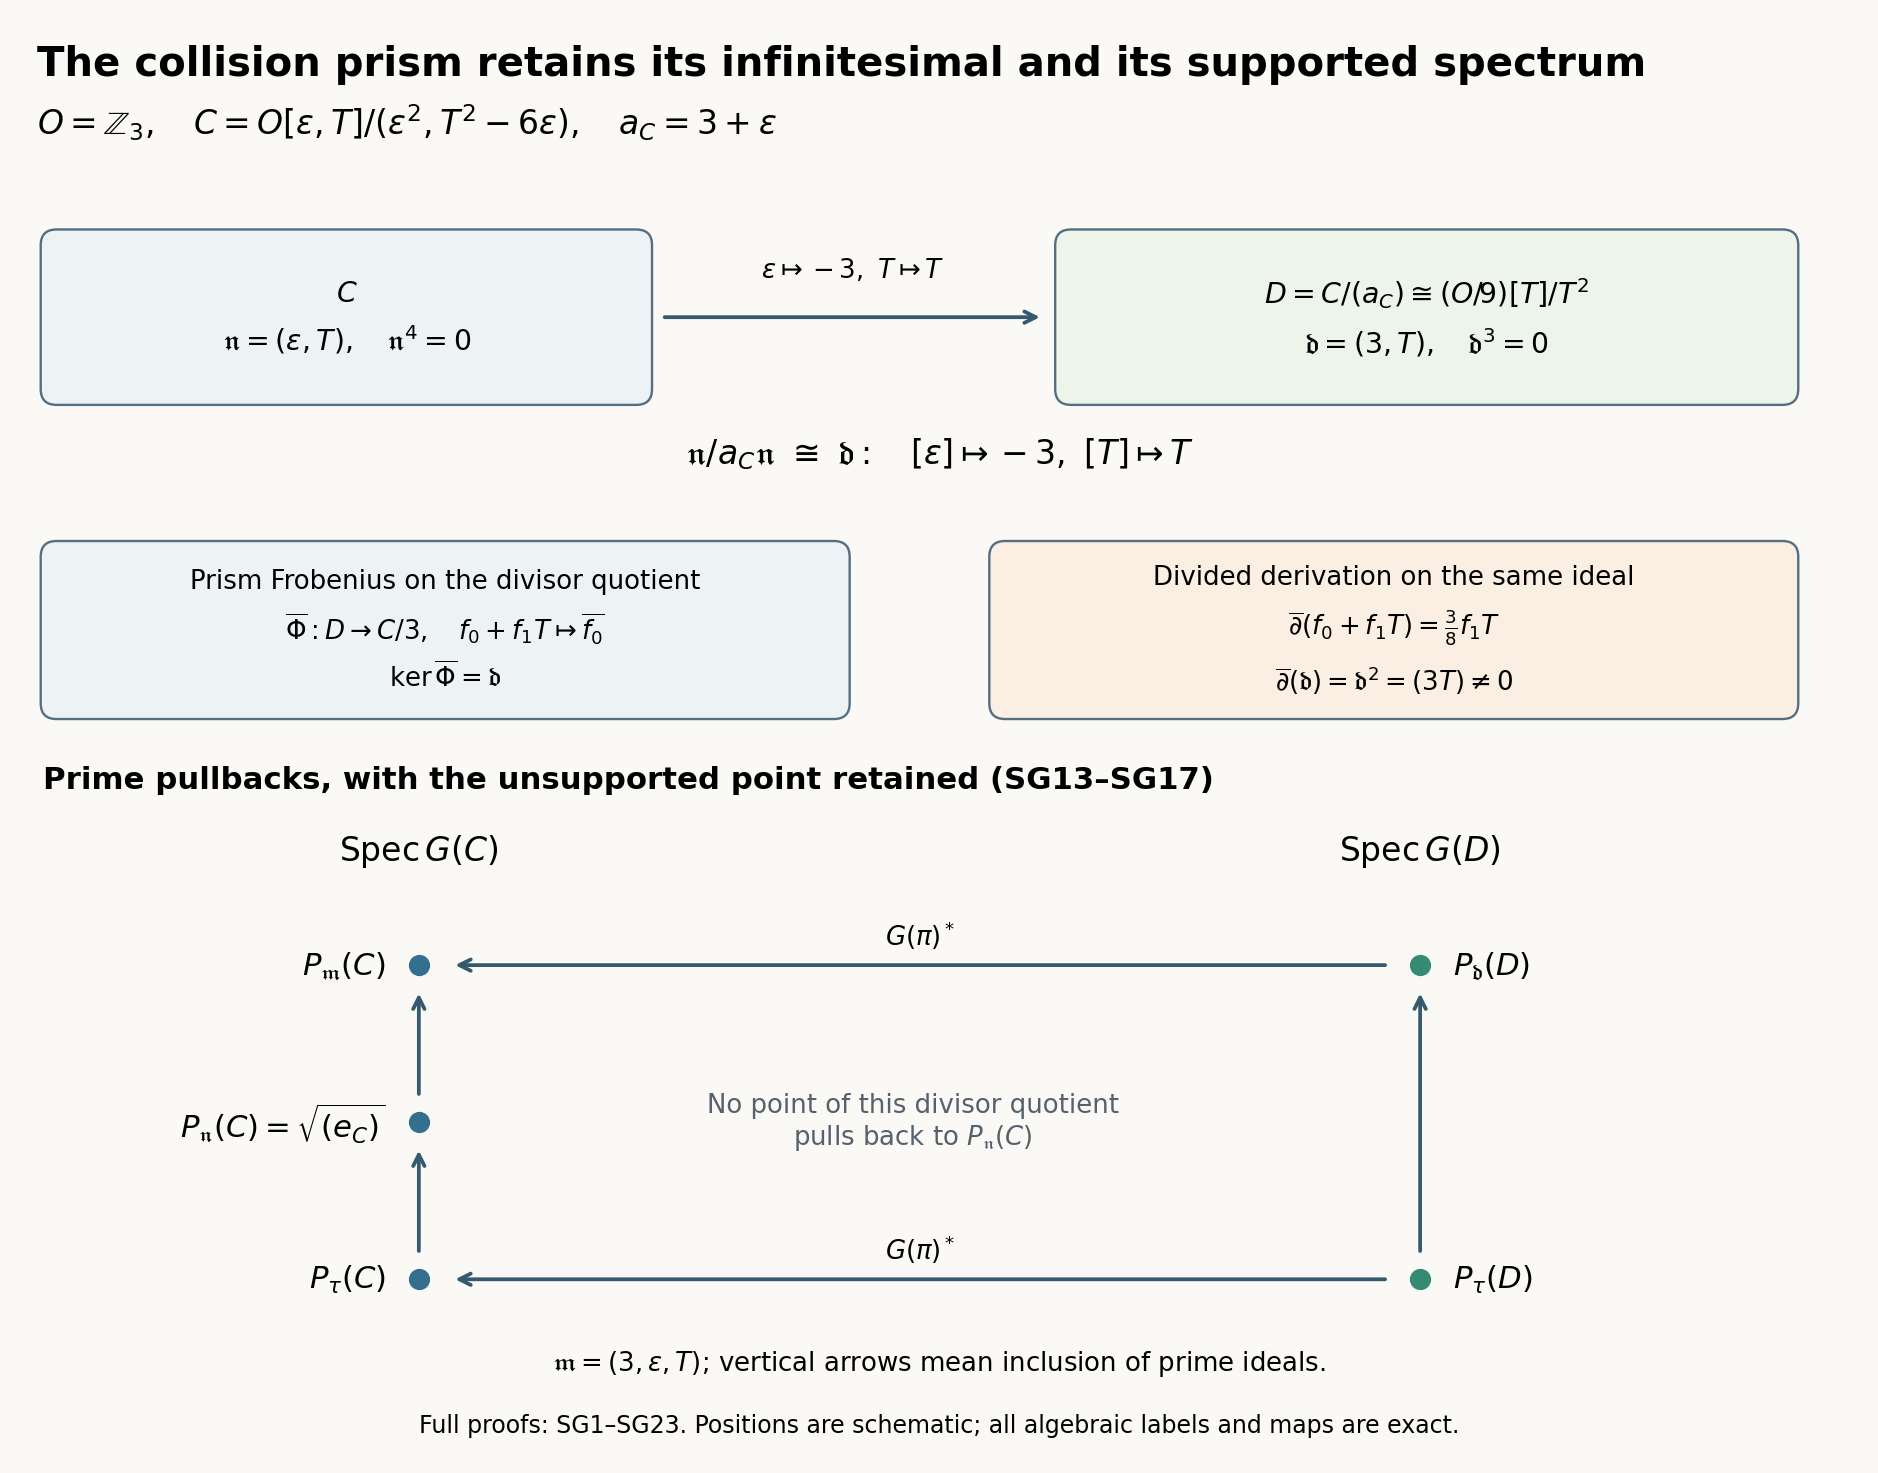
\includegraphics[keepaspectratio,alt={The divisor quotient and prime pullbacks, including the nonclosed supported image. The Frobenius kernel and divided-derivation image are ideals in the same ring. Full proofs SG13--SG23.}]{supported_collision_prism.png}}
\caption{The divisor quotient and prime pullbacks, including the
nonclosed supported image. The Frobenius kernel and divided-derivation
image are ideals in the same ring. Full proofs SG13--SG23.}
\end{figure}

\end{document}
